\documentclass[12pt]{article}
\usepackage[a4paper, margin=.30in]{geometry}
\usepackage{graphicx ,
            wrapfig,
            xcolor, 
            enumerate,
            amsmath,fontenc, mhchem
            }

\newcommand\headerMe[2]{\noindent{}#1\hfill#2}
\renewcommand{\thesection}{\Roman{section}}

\author{Zakaria HAOUZAN}
\date{\today}

\begin{document}
% headers --------------
\headerMe{Matière : Physique-Chimie}{Professeur : Zakaria HAOUZAN}\\
\headerMe{Unité : Transformations lentes et rapides\\ d'un système chimique }{Établissement : Lycée SKHOR qualifiant}\\
\headerMe{Niveau : 2BAC-SM-X}{Heure : 11H}\\

% ------Content ________
\begin{center}

    \Large{Leçon $N^{\circ} 2.2 $: \color{red} Suivi temporel d’une transformation - Vitesse de réaction }
\end{center}

%\begin{figure}[h!]
	%\begin{center}
	%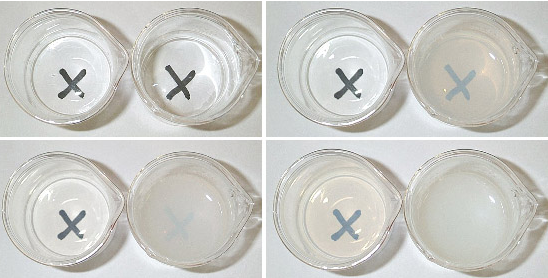
\includegraphics[width=0.5\textwidth]{./img/TRLconcentration.png}
%\end{center}
%\vspace{-1cm}
%\end{figure}



%\begin{wrapfigure}[10]{r}{0.5\textwidth}
%    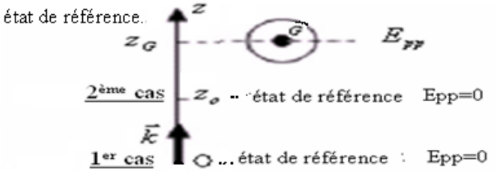
\includegraphics[width=0.5\textwidth]{./img/img00.png}
%\end{wrapfigure}


%\begin{center}
   %\begin{tabular}{|c|c|c|}
      %\hline
      %Indicateur coloré & Couleur de l’espèce acide & Couleur de l’espèce base\\\hline
      %BBT               & Jaune                     & Bleue\\\hline
      %Hélianthine       &Rose                       & Jaune\\\hline
      %Phénolphtaléine   & inclore                   & rose \\\hline
   %\end{tabular}
%\end{center}

\section{Techniques de suivi temporel d'une transformation :}

Pour suivre temporellement l'évolution d'une transformation chimique on doit connaître sa composition à chaque instant.
Il existe plusieurs méthodes qui permettent de suivre l'évolution d'une transformation chimique : 
\\- Le dosage.
- La conductimétrie.
- La mesure de la pression.
- La pH-métrie.

\begin{wrapfigure}[1]{r}{0.3\textwidth}
	\vspace{-3cm}
	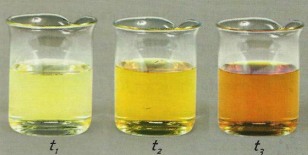
\includegraphics[width=0.27\textwidth]{./img/STidureavecperoxo.png}
\end{wrapfigure}



\section{suivi temporel d'une transformation :  }
\subsection{Le Dosage : }
\subsubsection{Expérience : }
Dans un bécher, verser 50 mL d'une solution incolore de peroxodisulfate de potassium, 
$(2K^+_{(aq)} + {S_2O_8^{2-}}_{(aq)})$, à $0,10 mol.L^{-1}$ puis 50 mL d'une solution, incolore elle aussi, d'iodure de potassium, $(K^+_{(aq)} +I^-_{(aq)})$.
à $0.50 mol.L^-$


\subsubsection{Exploitation :}
\begin{itemize}
	\item L'apparition progressive de la coloration jaune, caractéristique des molécules ${I_2}_{(aq)}$, montre que ces molécules sont formées par une réaction lente entre les ions peroxodisulfate ${S_2O_8}^{2-}$ et les ions iodure$I^-$. 

\item Les ions peroxodisulfate $S_2O_8^{2-}$ oxydent les ions iodure $I^-$ selon une réaction d'équation: 

	$2I^-_{(ag)} + {S_2O_8^{2-}}_{(aq)} = {I_2}_{(aq)} + 2{SO_4^{2-}}_{(aq)}$ (1)

	\item Cete réaction nétant pas trop rapide, elle peut être suivie en dosant le
diode formé.

\item On peut également utiliser la spectrophotométrie puisque la réaction met en jeu une seule espèce colorée, le diiode.

\item Les ions iodures $I^-$ sont lentement oxydés par les ions peroxodisulfate ce qui entraine la formation progressive du diiode $I_2$.
Pour savoir la quantité du diiode qui s'est formée à un instant donné on réalise le dosage de la manière suivante:

\item On recueille après chaque trois minutes $10cm^3$ du mélange réactionnel et on la trempe dans l'eau froide pour arrêter la réaction,Puis on dose le diiode $I_2$ formé par une solution de thiosulfate de sodium $(2Na^+ + {S_2O_3}^{2-})$  de concentration $Cr= 0,02mol/L$.


%\begin{figure}[h!]
	\begin{center}
	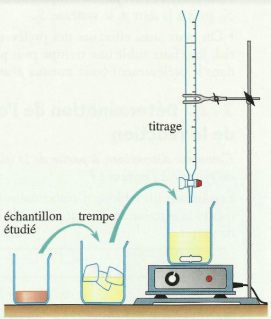
\includegraphics[width=0.3\textwidth]{./img/STlatrempe.png}
	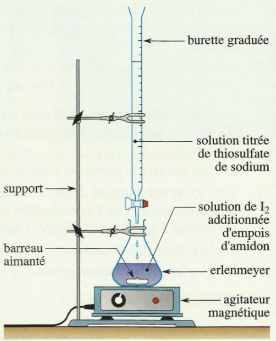
\includegraphics[width=0.3\textwidth]{./img/STmotageDosage.png}
\end{center}

%\end{figure}
\item Les deux couples mis en jeux durant le dosage sont :$I_2/I^-$ ET $S_4O_6^{2-}/S_2O_3^{2-}$.
\item Equation de la réaction du dosage: \ce{2S_2O_3^{2-} + I_2 -> S_4O_6^{2-} + 2I^-}
c'est une réaction rapide 
\item à l'équivalence : $\frac{n(S_2O_3^{2-})}{2} = \frac{n(I_2)}{1}$

\item Soit vr le volume de la solution de thiosulfate de sodium ajoutée à l'équivalence. $n(I_2) = \frac{C_r.V_r}{2}$

\item Tableau des mesures: 

\begin{center}
   \begin{tabular}{|c|c|c|c|c|c|c|c|c|c|c|c|}
	  \hline
	  t(s)         &0&3  &6&9&12&16&20&30&40&50&60 \\\hline
	  n($I_2 mmol$)&0&0.5&1.0 &1.4&1.7&2.1&2.3&2.8&3.1&3.2&3.3\\\hline
   \end{tabular}
\end{center}






\end{itemize}
\section{la prepatio}
fdswlfmkjsfdlm

\end{document}

